% !Mode:: "TeX:UTF-8"
\documentclass{../common/tufte-latex/tufte-handout}

\title{Git hands-on, part II: Single User Operations}
\author{S\'ebastien Dawans}

%\date{07 February 2014} % without \date command, current date is supplied

%\geometry{showframe} % display margins for debugging page layout
\usepackage[utf8]{inputenc}
\usepackage{graphicx} % allow embedded images
  \setkeys{Gin}{width=\linewidth,totalheight=\textheight,keepaspectratio}
  \graphicspath{{graphics/}} % set of paths to search for images
\usepackage{amsmath}  % extended mathematics
\usepackage{booktabs} % book-quality tables
\usepackage{units}    % non-stacked fractions and better unit spacing
\usepackage{multicol} % multiple column layout facilities
\usepackage{lipsum}   % filler text
\usepackage{fancyvrb} % extended verbatim environments
  \fvset{fontsize=\normalsize}% default font size for fancy-verbatim environments
\usepackage{listings}
\lstset{showstringspaces=false}
\usepackage[usenames]{xcolor}

\lstdefinestyle{BashInputStyle}{
  language=bash,
  basicstyle=\footnotesize\ttfamily,
  %numbers=left,
  %numberstyle=\tiny,
  %numbersep=3pt,
  frame=tb,
  columns=fullflexible,
  backgroundcolor=\color{yellow!20},
  linewidth=0.95\linewidth,
  xleftmargin=0.05\linewidth,
  moredelim=**[is][\color{red}]{§}{§},
  moredelim=**[is][\color{OliveGreen}]{`}{`}
}

% Standardize command font styles and environments
\newcommand{\doccmd}[1]{\texttt{\textbackslash#1}}% command name -- adds backslash automatically
\newcommand{\docopt}[1]{\ensuremath{\langle}\textrm{\textit{#1}}\ensuremath{\rangle}}% optional command argument
\newcommand{\docarg}[1]{\textrm{\textit{#1}}}% (required) command argument
\newcommand{\docenv}[1]{\textsf{#1}}% environment name
\newcommand{\docpkg}[1]{\texttt{#1}}% package name
\newcommand{\doccls}[1]{\texttt{#1}}% document class name
\newcommand{\docclsopt}[1]{\texttt{#1}}% document class option name
\newenvironment{docspec}{\begin{quote}\noindent}{\end{quote}}% command specification environment

\begin{document}

\maketitle% this prints the handout title, author, and date

\begin{abstract}
\noindent
This handout complements the information given in the previous handout, \textbf{part I: single user operations}.
The first part looks at how to ignore files from Git.
The rest documents the history modification commands that were introduced orally during the last session in answer to specific questions.
\end{abstract}


\section{Exploring the Repository}

So we have just cloned out first repository, and have seen the difference between the \textbf{working tree} and \textbf{local repository}.
Most of the git commands we use will interact with the local git repository to write and read information to and from the working tree.
Before we actually change anything, let's take a look at the commands available to browse the current status of a project and its history.

\subsection{Listing Remotes}

The \texttt{git clone} command initiated a local repository replicating a \textbf{remote} repository, identified by a URL.
Information related to the state of \textbf{remote} repostories is stored in a dedicated area within the Git repository.
For a name-only list of remotes, we use:

\begin{lstlisting}[style=BashInputStyle]
  $ git remote
  origin
\end{lstlisting}

Every remote is identified by a short-hand name: \textbf{origin} in this case which is the default name Git assigns to a remote when it is cloned.
We can rename a remote repository to give it a more expressive name.
Let's rename it to \texttt{gitlab}, to remind us that the remote is hosted on our local Gitlab server.

\begin{lstlisting}[style=BashInputStyle]
  $ git remote rename origin gitlab
\end{lstlisting}


There is a verbose version of \texttt{git remote} which lists the URLs to each remote.
\marginnote{There are actually 2 URLs defined for each remote, allowing to decouple \texttt{fetch} from \texttt{push} to use different protocols or even different paths for some very specific configurations.}

\begin{lstlisting}[style=BashInputStyle]
  $ git remote -v
  gitlab  git@gitlab.server.com:login/lesson1 (fetch)
  gitlab  git@gitlab.server.com:login/lesson1 (push)
\end{lstlisting}

We will get back to remotes later, let's just mention that it is possible to add and delete a remote, as well as set a new URL for an existing remote.
For example, we can set an altenate but equivalent notation of the URL:

\marginnote{This is a 1-line command displayed in 2 lines for readability. I use the "\textbackslash" character and an indented second line to represent this.}

\begin{lstlisting}[style=BashInputStyle]
  $ git remote set-url gitlab \
     ssh://git@gitlab.server.com:login/lesson1.git
\end{lstlisting}

\subsection{Local and Remote branches}

As we will see throughout this course, \textbf{branches} are omnipresent in Git.
Therefore, commands which list branches and show their relationships are particularly useful.
The simplest way to list branches is:

\marginnote{Omitting the \texttt{-a} option of \texttt{git branch} will display only the local branches.}

\begin{lstlisting}[style=BashInputStyle]
  $ git branch -a
  * `master`
  §remotes/origin/HEAD -> origin/master§
  §remotes/origin/master§
\end{lstlisting}

The output lists local and remote branches.
The local branches are first displayed in default color, with the exeption of the \textbf{currently checked-out} branch, which is displayed in green and has an asterisk next to it.
Here, the current branch is master.

The remote branches are displayed in red and are prefixed with \texttt{remotes/alias/} for readability.
There's a special \texttt{HEAD} pointing on a remote branch which simply identifies the remote branch set as the project's default branch, which will be checked out locally when doing a \texttt{git clone}.

\subsection{Viewing the history}

To view the history of the current branch:

\begin{lstlisting}[style=BashInputStyle]
  $ git log
\end{lstlisting}

This will display a verbose output of the log in a scrollable text viewer.
\marginnote{The log manpage \texttt{git log --help} is a great reference as well as online resources such as \url{http://gitready.com/advanced/2009/01/20/bend-logs-to-your-will.html}
\\ \vspace{0.5cm}
\noindent The last command shows a textual graph of the history. A useful and complete git log graph is given at \url{http://stackoverflow.com/questions/1057564/pretty-git-branch-graphs}}
Git log has plenty of useful options, I will list a few of them here and let you experiment with them.

\begin{lstlisting}[style=BashInputStyle]
  $ git log -n 3
  $ git log --pretty=oneline
  $ git log --pretty=[short, medium, full, fuller, raw...]
  $ git log --pretty=format:'%h - %d %s (%cr) <%an>'
  $ git log --pretty=format:'%h -%C(red)%d%C(reset) %s (%cr) <%an>'
  $ git log --oneline
  $ git log --since "3 hours ago"
  $ git log --since "1 week ago"
  $ git log --graph --pretty=format:' ... '
\end{lstlisting}

\subsection{Graphical overview of branches}

We have seen that there are command-line ways of comparing commits in branches with textual graphs, but this can get complicated when dealing with multiple branches and remotes.
An alternative is to use a graphical user interface, such as Gitk which is distributed in msysgit and included in Linux and MacOS X installations.
To open Gitk:

\begin{marginfigure}%
  \centering
  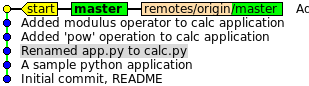
\includegraphics[width=\linewidth]{gitk-start.png}
  \label{fig:gitk-start}
  \caption{Our very simple project displayed in Gitk. There is only 1 local branch with a linear history.}
\end{marginfigure}

\begin{lstlisting}[style=BashInputStyle]
  $ gitk --all
\end{lstlisting}

This is by far the fastest and easiest way to get an overview of the local and remote branches.
In Gitk, the local branches are green, the current local branch is green and bold, and remote branches are prefixed with a peach path.
Our project also has a yellow label, which is a tag.
Like a branch, a \texttt{tag} is little more than a label on a certain commit, the main difference being that a tag is designed to be permanent to label an important point in the project history for future reference (code release, development milestone...), whereas a branch is meant to evolve.
We'll get back to branches and tags later.

\subsection{Working tree status}

We are about to start applying changes to our project.
A useful command to track the status of the different files in Git is \texttt{git status}:

\begin{lstlisting}[style=BashInputStyle]
  $ git status
\end{lstlisting}

As we have not yet modified anything, our git status output is very short:

\begin{lstlisting}[style=BashInputStyle]
  On branch master
  nothing to commit (working directory clean)
\end{lstlisting}

Git status is more verbose when you start changing things.
It will group files in categories according to their state: \textbf{staged}, \textbf{modified} and \textbf{untracked}.

\section{Applying our first changes to master}
In many workflows, it is usually not recommended to work directly on the master branch.
We will do so only this first time to keep things simple.
In the future, we will always apply modifications in isolated branches, and bring these changes back onto master if desireable.

\subsection{Git add to stage an untracked file}

Let's create a new file and see the output of git status:

\begin{lstlisting}[style=BashInputStyle]
  $ echo hello > newfile.txt
  $ git status
  # On branch master
  # Untracked files:
  #   (use "git add <file>..." to include in what will be committed)
  #
    §newfile.txt§
  nothing added to commit but untracked files present (use "git add" to track)
\end{lstlisting}

Git status is more verbose, it tells us that there's untracked content inside the working tree.
All files added to a git working tree are untracked, and will stay untracked unless explicitly defined as tracked content in the repository.

\begin{marginfigure}%
  \centering
  
\includegraphics[width=\linewidth]{gitadd-schema.pdf}
  \label{fig:gitadd}
  \caption{Git add on a file will stage all modifications in the file. It also adds untracked files to the staging area.}
\end{marginfigure}

\begin{lstlisting}[style=BashInputStyle]
  $ git add newfile.txt
  $ git status
    On branch master
    Changes to be committed:
      (use "git reset HEAD <file>..." to unstage)
  
    `new file:   newfile.txt`
\end{lstlisting}

\subsection{Our first commit}

The staging area is unique to Git, and makes it very powerful.
\marginnote{The term commit is also used in SVN, but it is very different here. An SVN commit is non-reversible and applies changes on the remote repository. A Git commit is a local operation and can easily be undone and edited before it reaches a remote server.}
Successive modifications can be applied until the developer is satisfied with the changes, and is ready to commit them.
Committing changes will define a new point in the project history with a description, and move the HEAD and current branch to the new commit.

\begin{marginfigure}%
  \centering
  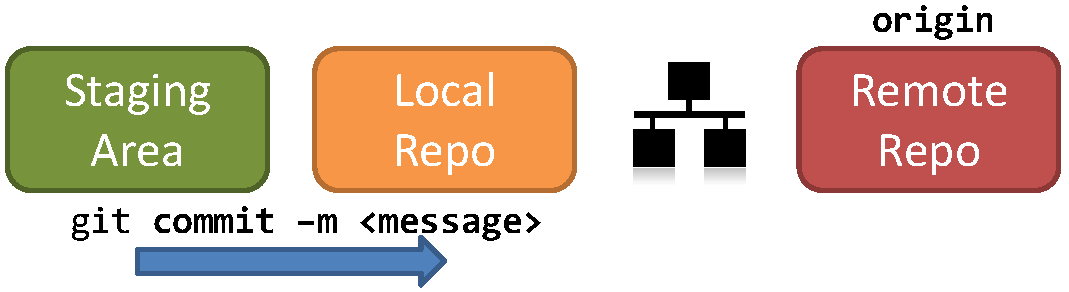
\includegraphics[width=\linewidth]{gitcommit-schema.pdf}
  \label{fig:gitcommit}
  \caption{Git commit creates a new point in history, applying the changes in the staging area.}
\end{marginfigure}

\begin{lstlisting}[style=BashInputStyle]
  $ git commit -m "Added new file"
  [master 494822d] Added new file
   1 file changed, 1 insertion(+)
   create mode 100644 newfile.txt
\end{lstlisting}

Above, the commit message is given inline with the \texttt{-m} option, but it may be entered via the default text editor by omitting this option.

\subsection{Git add to stage modifications in tracked files}

Let's add more content to our new file and commit these changes.

\begin{lstlisting}[style=BashInputStyle]
  $ echo "hello again" >> newfile.txt
  $ git status
    On branch master
    Your branch is ahead of 'origin/master' by 1 commit.
  
    Changes not staged for commit:
      (use "git add <file>..." to update what will be committed)
      (use "git checkout -- <file>..." to discard changes in working directory)
   
    §modified:   newfile.txt§
   
no changes added to commit (use "git add" and/or "git commit -a")
\end{lstlisting}

Typing \texttt{git commit} at this point will not apply anything, because the modifications have not been added to the staging area.
It is possible to apply changes on a file basis in the same way as we have staged an untracked file previously:

\begin{lstlisting}[style=BashInputStyle]
  $ git add newfile.txt
  $ git status
    On branch master
    Your branch is ahead of 'origin/master' by 1 commit.
  
    Changes to be committed:
      (use "git reset HEAD <file>..." to unstage)
  
    `modified:   newfile.txt`
 
\end{lstlisting}

Committing now will apply the modifications.

\begin{marginfigure}%
  \centering
  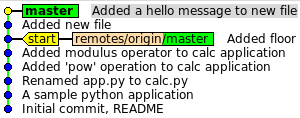
\includegraphics[width=\linewidth]{gitk-2commits.png}
  \label{fig:gitk2commits}
  \caption{Gitk after 2 commits on the local master branch}
\end{marginfigure}

\begin{lstlisting}[style=BashInputStyle]
  $ git commit -m "Added a hello message to new file"
  [master 25d79d3] Added a hello message to new file
   1 file changed, 1 insertion(+)
\end{lstlisting}

\subsection{Git add -p: content-based staging}

Probably the cleanest way to stage changes in Git is to use the \texttt{-p} option of \texttt{git add}:

\begin{lstlisting}[style=BashInputStyle]
  $ git add -p
\end{lstlisting}

This doesn't require any files as argument.
\texttt{git add -p} will initiate an interactive session during which each modification will be displayed, and the user must decide whether to add the changes to the staging area, or leave it as modified. \marginnote{\texttt{git add -p} common commands: \textbf{y}: stage, \textbf{n}: do not stage, \textbf{d}: don't stage and skip rest of file, \textbf{s}: split into smaller chunks and ask again.}
The great thing about this command is that the modifications are presented per line (or groups of adjacent lines) rather than by file, meaning that you can stage a part of a file without staging the rest of it.
That way, it's very easy to isolate features in different commits, even if these involve modification in the same set of files.
The interactive prompt will end when all changes have been cycled through.

Suppose I have made two modifications in \texttt{calc.py} and that I have selected \textbf{y} for only one of these when running \texttt{git add -p}.
The file with contain both staged and modified lines:

\begin{lstlisting}[style=BashInputStyle]
  $ git status
    On branch master
    Your branch is ahead of 'origin/master' by 2 commits.
  
    Changes to be committed:
      (use "git reset HEAD <file>..." to unstage)
  
    `modified:   python/calc.py`
  
    Changes not staged for commit:
      (use "git add <file>..." to update what will be committed)
      (use "git checkout -- <file>..." to discard changes in worki...
  
    §modified:   python/calc.py§
\end{lstlisting}

Git commit at this point will apply the staged code to the commit, and leave the file in the modified state with the remaning, unstage lines.
We have already covered commits, so let's stay in this state to explore the \textbf{diff} command.

\marginnote{\texttt{git diff} will display the full diff between the modified content and HEAD. Already staged data does not appear.}
\begin{lstlisting}[style=BashInputStyle]
  $ git diff
  diff --git a/python/calc.py b/python/calc.py
  index b66135e..9178e52 100644
  --- a/python/calc.py
  +++ b/python/calc.py
  @@ -17,6 +17,7 @@ def mul(op1, op2):
   def div(op1, op2):
     return op1 / op2
 
  `+ New comment, I will not stage it for now`
   def pow(op1, op2):
     return op1 ** op2
 \end{lstlisting}
\marginnote{\texttt{git diff} with the \textbf{cached} option is the opposite: it displays the diff between the staged content and HEAD, and ignores modified content.}
 \begin{lstlisting}[style=BashInputStyle]
  $ git diff --cached
  diff --git a/python/calc.py b/python/calc.py
  index c27b82f..b66135e 100644
  --- a/python/calc.py
  +++ b/python/calc.py
  @@ -2,6 +2,7 @@ import os
   import sys
   import argparse
 
  `+ New comment. I will stage this first`
   choices_cmd = ['add', 'sub', 'mul', 'div', 'pow', 'mod', 'floor']
 
   def add(op1, op2):
\end{lstlisting}

\subsection{Stage all modified and untracked in 1 command}

I recommend avoiding this as much as possible, but for the record, it is possible to use a single command to add all untracked and modified files to the staging area:

\begin{lstlisting}[style=BashInputStyle]
  $ git add -A
\end{lstlisting}

\subsection{Commit all modified files in 1 command}

Another shortcut worth knowing but which should be avoided in most cases is the commit option to stage all outstanding modifications and record a new commit:
\begin{marginfigure}%
  \centering
  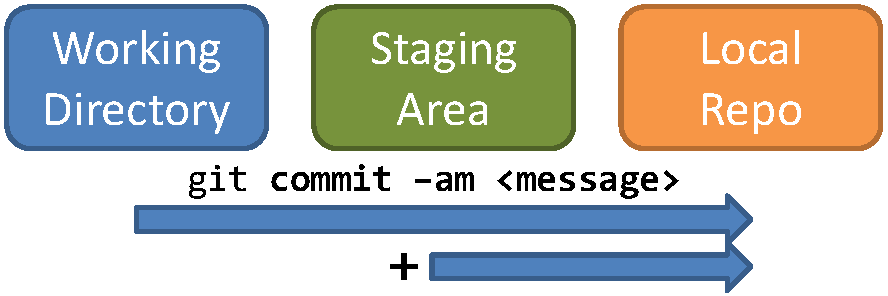
\includegraphics[width=\linewidth]{gitcommit-am-schema.pdf}
  \label{fig:gitcommit-am}
  \caption{Git commit -am stages all modified files and applies a commit immediately after.}
\end{marginfigure}
\begin{lstlisting}[style=BashInputStyle]
  $ git commit -am "One big commit"
\end{lstlisting}

I prefer avoiding this because commits should be decoupled by features and it is rare that there are no superfluous modifications when developing a feature.
This \texttt{-a} option doesn't leave time to verify the contents of the commit before applying changes, whereas decoupling staging and commit phases allows to view the staged changes with commands like:

\begin{lstlisting}[style=BashInputStyle]
  $ git diff --cached
\end{lstlisting}

\subsection{Unstaging stuff}

To unstage work, \texttt{git reset} comes in handy.
This command is very multi-purpose in Git, for now we will use its default behavior which is to unstage modifications without deleting them.
\texttt{git reset} without arguments will unstage all currently staged changes, and bring them back to their former state (modified or untracked).

\marginnote{Although it's technically possible to combine \texttt{[tree-ish]} and \texttt{[file]} options to git reset, this will not actually delete the commit if there are other non-reset changes in the commits. Thus the content is reset as desired, but applied this reset requires to stage and commit the modifications in new commits. Git revert has a similar behavior in the sense that we are adding commits to actually undo work.}

\begin{lstlisting}[style=BashInputStyle]
  $ git reset 
\end{lstlisting}

This is only a partial explanation of why git reset does this.
Like many git commands which accept a \textbf{tree-ish} as optional argument, git reset assumes \texttt{HEAD} when unspecified.
The general \texttt{git reset} actually undoes commits from the current state up until (and not including) the commit referenced by the tree-ish.

\begin{lstlisting}[style=BashInputStyle]
  $ git reset [tree-ish]
\end{lstlisting}

Finally, unstaging can also be applied on a per-file basis.

\begin{lstlisting}[style=BashInputStyle]
  $ git reset [file]
\end{lstlisting}

\section{Untracking and Deleting files}

Deleting a file is treated in the same way as other modifications in Git.
There are two ways to remove a file from version control.
The \textit{clean and recommended} way consists in invoking the file/folder removal directly with Git.
Removing content directly from the filesystem is not as clean, but is \textbf{easily recoverable} in Git.
\marginnote{SVN users: yes, that my sound like magic.}
We will have a look at both methods in this section.

\subsection{Removing files using Git}

The cleanest way to remove a file from disk as well as from the Git repository is to use \texttt{git rm} on it:

\begin{lstlisting}[style=BashInputStyle]
  $ git rm <file>
\end{lstlisting}

This performs two things: it deletes the file from disk, and \textbf{stages} the removal of this file.
The next commit will thus include the deletion of the file.

If you want to untrack a file from Git \textit{without deleting it} locally, use the \texttt{cached} option:

\begin{lstlisting}[style=BashInputStyle]
  $ git rm --cached <file>
\end{lstlisting}

\marginnote{rm cached comes in very handy to untrack things you forgot to add to your .gitignore file}
Git will stage the file to be removed in the next commit, but will not touch the file locally.

\subsection{Removing files outside of Git}

So, what happens when you delete some content locally that Git has been versioning?
Git will detect the missing content, as a \texttt{git status} will tell you:

\begin{lstlisting}[style=BashInputStyle]
  $ rm README.md
  $ git status
  On branch master
  Your branch is up-to-date with 'origin/master'.

  Changes not staged for commit:
    (use "git add/rm <file>..." to update what will be committed)
    (use "git checkout -- <file>..." to discard changes in working directory)

      §deleted:    README.md§

  no changes added to commit (use "git add" and/or "git commit -a")
\end{lstlisting}

\marginnote{as opposed to a git rm README.md, which stages the deletion.}
The deleted content is equivalent to a modification: it is not staged by default.
It is possible to execute \textit{git rm} on each deleted file, even though it's not on disk anymore, which will tell git to stage the deletion.
However, this can be tedious if you've removed lots of files.
Instead, you can ask git to synchronize the staging area with all modified content with:

\begin{lstlisting}[style=BashInputStyle]
  $ git add -u
\end{lstlisting}

In case of deleted files, \texttt{git add -u} will stage every modification at once.
The next commit will apply the file removals.

\pagebreak

\section{Pushing work to a remote}

We have progressed locally on the master branch.
So far, all our modifications are local and we have not shared our work with anyone.

\begin{marginfigure}%
  \centering
  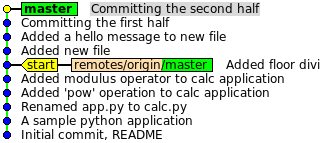
\includegraphics[width=\linewidth]{gitcommit-pre-push.png}
  \label{fig:gitcommit-pre-push}
  \caption{Local and remote repo status before the push. Local master is 4 commits ahead of origin's.}
\end{marginfigure}
\begin{marginfigure}%
  \centering
  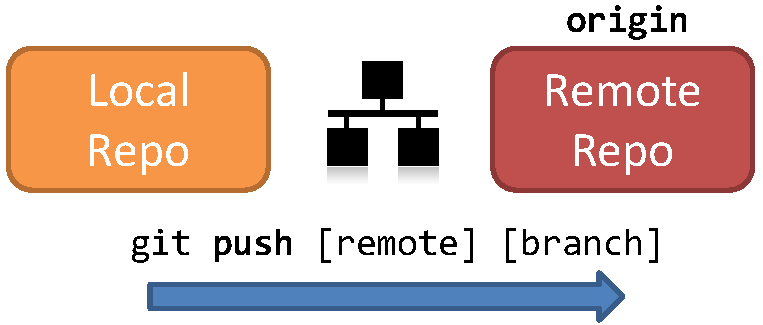
\includegraphics[width=\linewidth]{gitpush-schema.pdf}
  \label{fig:gitpush-schema}
\end{marginfigure}
\begin{marginfigure}%
  \centering
  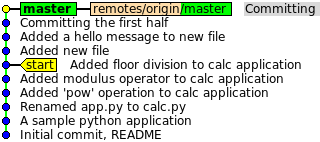
\includegraphics[width=\linewidth]{gitcommit-post-push.png}
  \label{fig:gitcommit-post-push}
  \caption{After pushing master to origin, both branches are at the same point in history.}
\end{marginfigure}

The \texttt{git push} command is used to push individual branches from the local repository to a remote one.
The command produces the following output.

\begin{lstlisting}[style=BashInputStyle]
  $ git push origin master 
  Counting objects: 17, done.
  Delta compression using up to 8 threads.
  Compressing objects: 100% (10/10), done.
  Writing objects: 100% (14/14), 1.29 KiB, done.
  Total 14 (delta 4), reused 0 (delta 0)
  To git@gitlab.server.com:login/lesson1
     71aaf45..37b9258  master -> master
\end{lstlisting}

Git push is only possible if the remote branch to which we are pushing has not been updated in the meantime.
In other words, it succeeds \textit{if the remote branch is in the direct history of the local branch}.

If pushing is not possible because the remote branch has been updated (usually, by someone else), we enter a multi-user workflow which we will cover later.
\marginnote{I use integrate here to stay general. There are many ways to do this, like merge, rebase, hard reset...}
In a few words, the remote modifications must first be \textbf{fetched} locally and "integrated" in our work before we can contribute.

\section{Applying our changes to a feature branch first}

So far we have worked on a master branch.
We will conclude this first session by working in feature branches, and merging them into the master branch once they are stable.

\subsection{Branching: very lightweight}

Branching in Git is as simple as adding a new label to an existing commit.
\marginnote{This is very different from some other SCMs, where creating a branch is a lengthy process involving copying the entire working tree.}
The working tree is left entirely intact when a branch is created.
\begin{marginfigure}%
  \centering
  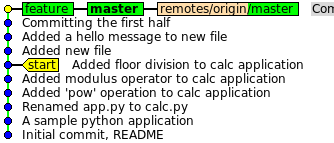
\includegraphics[width=\linewidth]{gitbranch-feature.png}
  \label{fig:gitbranch-feature}
  \caption{A new branch is just a new label.}
\end{marginfigure}
\begin{lstlisting}[style=BashInputStyle]
  $ git branch -a
  * `master`
    §remotes/origin/HEAD -> origin/master§
    §remotes/origin/master§

    $ git branch feature

  $ git branch -a
    feature
  * `master`
    §remotes/origin/HEAD -> origin/master§
    §remotes/origin/master§
\end{lstlisting}

We have a new local branch called feature branch, currently pointing to the same commit as master.
We are not quite ready to start applying changes, because \texttt{git branch} and \texttt{git status} tell us that we are still in master.
To progress in the \texttt{feature} branch rather then \texttt{master} we must use \textbf{checkout}:

\begin{lstlisting}[style=BashInputStyle]
  $ git checkout feature
  $ git branch -a
  * feature
    master
    remotes/origin/HEAD -> origin/master
    remotes/origin/master
\end{lstlisting}

\subsection{Integrating a feature branch back into master}

Now, we can start adding commits to the feature branch just like we have done for master.
Once we are satisfied with our work, we can merge it back into master.
We will not go into too much details for now, but the general idea is:

\begin{marginfigure}%
  \centering
  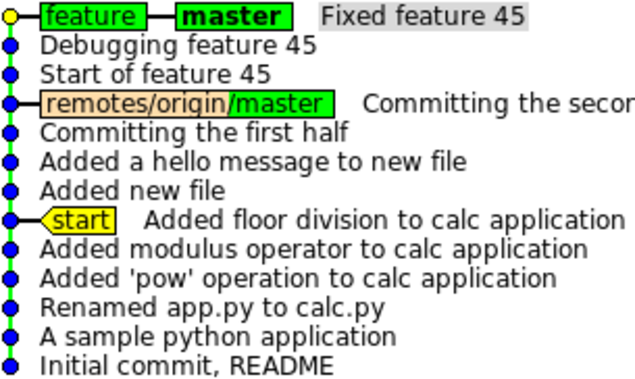
\includegraphics[width=\linewidth]{gitmerge-ff.pdf}
  \label{fig:gitmerge-ff}
  \caption{Merging in fast-forward mode.}
\end{marginfigure}

\begin{lstlisting}[style=BashInputStyle]
  $ git checkout master
  $ git merge feature
\end{lstlisting}

If master has not progressed since we branched off with feature, the master branch will be \textbf{fast-forwarded} to the feature branch.
If a branching history is preferred, we can force it with \texttt{no-ff}:

\begin{marginfigure}%
  \centering
  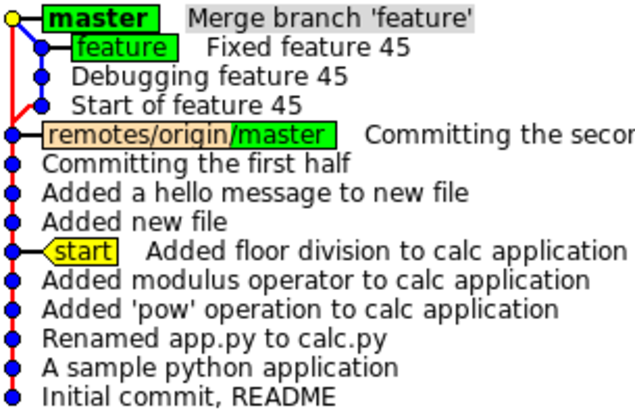
\includegraphics[width=\linewidth]{gitmerge-noff.pdf}
  \label{fig:gitmerge-noff}
  \caption{Merging in no-fast-forward mode creates an explicit merge commit.}
\end{marginfigure}

\begin{lstlisting}[style=BashInputStyle]
  $ git checkout master
  $ git merge feature --no-ff
\end{lstlisting}

This creates an additional commit, called a merge commit, with 2 parents: the last commit on each branch prior to the merge.
If master \textit{did} progress since we branched off with the feature branch, the merge operation will automatically result in an extra merge commit.

\section{Ignoring files}
In many source code directories, there are files which we do not want to (or should not) version control.
Any file which is generated from source code and likely to change at every compilation of the project should not be version controlled.
Likewise, huge files should be handled by other means, even if these are not necessarily regenerated and are a required dependency for a project compilation or runtime like a library.
To handle this, Git can be told to ignore certain files by pattern rules.
Ignored untracked files will stay untracked without polluting the \textbf{git status} output.

\subsection{Using .gitignore files}
There are several ways of instructing git to ignore files by pattern rules, the most common one is by means of \textbf{.gitignore} files placed in the working tree and version-controlled in the same way as a normal file.
\marginnote{Type \textbf{git help gitignore} for a list of other ways to ignore files. Note that there is an order of precedence.}

It is important to define a \textbf{.gitignore} file as early on in a Git project as possible.
When creating a new project from scratch, it's good practice to include a .gitignore file in the first commit, even if empty.
When adding an existing code base to Git, it's even more important to get the .gitignore right before adding the whole project recursively, because there might already exist some files which you need to ignore.

\noindent \textbf{Example}.
Consider a very simple C project with .c files, a Makefile and a generated binary.
Suppose we have just created a \texttt{hello.c} file, adapted our Makefile and compiled it:

\begin{lstlisting}[style=BashInputStyle]
  $ git status
  On branch master
  Untracked files:
    (use "git add <file>..." to include in what will be committed)
  
      §Makefile§
      §hello.c§
      §hello.exe§

nothing added to commit but untracked files present (use "git add" to track)
\end{lstlisting}

If we type \texttt{git add .} at this point, all three files will be added to Git.
Suppose we wanted to ignore the generated file, we could decide to exlude all files ending in ".exe", let's create a file called .gitignore and add \textbf{*.exe} on the first line:
\begin{lstlisting}[style=BashInputStyle]
  $ touch .gitignore
  $ echo "*.exe" >> .gitignore
\end{lstlisting}

The next time we look at \texttt{git status}, it will be ignored:
\begin{lstlisting}[style=BashInputStyle]
  $ git status
  On branch master
  Untracked files:
    (use "git add <file>..." to include in what will be committed)
  
      §.gitignore§
      §Makefile§
      §hello.c§

nothing added to commit but untracked files present (use "git add" to track)
\end{lstlisting}

Notice that we have a new untracked file, our new .gitignore file.
We can now add the whole project and make our first commit.

\begin{lstlisting}[style=BashInputStyle]
  $ git add .
  $ git commit -m "Initial Commit: adding the project files"
\end{lstlisting}

In Git the .gitignore files are part of the working tree and must be committed like any other source file.
This is very convenient because it allows to propagate the rules of ignored files.
Regular users of a project thus do not usually worry about .gitignores, the work of defining ignored files having already been done by the project owner, who knows best which files should be ignored.

\subsection{Forgot to ignore some files?}
At some point you might forget to include a certain pattern in a .gitignore.
If some files have accidentally been added to version control when they should not have, it is easy to ignore them later.
Assuming that the file is not required to be on the repository, we have already learned the required command in the previous lesson: \texttt{git rm} with the \texttt{cached} option.

Suppose we have a \texttt{hello.exe} binary file part of the repository which we want to untrack and ignore, we would do:
\marginnote{The \textbf{cached} option preserves a local copy of hello.exe, which isn't really necessary since we know we can just regenerate it with our Makefile}
\begin{lstlisting}[style=BashInputStyle]
  $ git rm --cached hello.exe
  $ echo "*.exe" >> .gitignore
  $ git add .gitignore
  $ git commit -m "Remove file hello.exe and ignore all *.exe files"
\end{lstlisting}

Note that this procedure is \textbf{not sufficient if you are concerned with removing a huge binary file from a git repository} for performance reasons, because it is still contained in the history and the blob in the git objects database is still there.
Permanently removing the objects from the repository requires all the refs on the blob to be removed, followed by a garbage collection of the unreferences blobs.
This is not trivial and definately out of scope of our lesson.

\subsection{Ignoring a versioned file without removing it from Git}
In some projects, it is sometimes necessary to ignore local modifications of a certain file but not remove the file from version control.
An example of this is when a developer needs to change parts of a file to match a certain local setting, like activating a debugging flag in a file or specifiying credentials like database login/password in a script interacting with a database.
Ignoring modifications to such files cleans your git status and also avoid you to accidentally commit those changes if you use shortcuts like \texttt{git commit -a}.
You cannot simply use a local (untracked) .gitignore file for this, because \textbf{.gitignore only applies to untracked files}; you cannot ignore a file already part of the repository.
\marginnote{A local, uncommitted .gitignore file would not be a clean way even if it was possible, because the .gitignore file itself would appear as untracked every time you type git status.}

Although git stash does the trick, git stash will actually hide your modifications from the working tree so you would need to stash and unstash your local modifications everytime you want to commit.

An simpler alternative is to temporarily ignore local changes in a file:
\begin{lstlisting}[style=BashInputStyle]
  $ git update-index --assume-unchanged <file>
\end{lstlisting}

This activates a certain flag on the file and marks it as ignored by Git.
The file will still receive updates from upstream, but local modifications will be ignored.
To undo this:

\begin{lstlisting}[style=BashInputStyle]
  $ git update-index --no-assume-unchanged <file>
\end{lstlisting}

You can obtain a list of all files ignore in this way using:

\begin{lstlisting}[style=BashInputStyle]
  $ git ls-files -v | grep ^[a-z]
\end{lstlisting}

The following 3 aliases are useful to add in your ~/.gitconfig:

\begin{lstlisting}[style=BashInputStyle]
[alias]
        ignore = !git update-index --assume-unchanged 
        unignore = !git update-index --no-assume-unchanged
        ignored = !git ls-files -v | grep ^[a-z]
\end{lstlisting}

\section{Rewriting History}
Git gives lots of power to the user and allows to rewrite the history.
This can be \textbf{rewording} commit messages, \textbf{combining} commits, \textbf{splitting} a large commit into smaller ones, \textbf{deleting} a commit, \textbf{reordering} commits, changing the \textbf{date and authoring} information, etc.

\noindent \textbf{Warning}. Changing the history of a branch which has already been shared to other people is not a good practice, because those people will have to hard reset their work to your new branch and apply their modifications on top of it.
\marginnote{Rewriting history is a great way of cleaning one's work before pushing, but should not be used a posteriori on an important branch (master, develop).}
If you ever have doubts about when it is ok or not to rewrite history, use this simple \textbf{rule: do not modify history pushed on a shared repository}.

\subsection{Amending the last commit}
The simplest form of history modification is changing the last commit:

\begin{lstlisting}[style=BashInputStyle]
  $ git commit --amend
\end{lstlisting}

This command opens up the last commit message, and allows you to alter the message.
It then takes whatever is in the staging area and adds it to the previous commit, with the new commit message, instead of creating a new commit.
Thus, this is for both \textbf{rewording the last commit} and \textbf{appending more changes to the last commit}.

Let's reword the last commit message of lesson1 in its initial state:

\begin{lstlisting}[style=BashInputStyle]
  $ git clone git@gitlab.server.com:login/lesson1
  $ cd lesson1
  $ git log --oneline
  $ gitk --all
  $ git commit --amend -m "New message"
  $ git log --oneline
  $ gitk --all
\end{lstlisting}

\begin{figure*}%
  \centering
  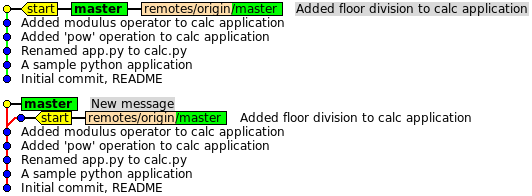
\includegraphics[width=0.85\linewidth]{gitcommit-amend.png}
  \label{fig:gitcommit-amend}
  \caption{Before (top) and after (bottom) amending the last commit message}
\end{figure*}

The output of gitk at the 2 steps is shown in Figure \ref{fig:gitcommit-amend}.
We can see that ammending the commit creates a divergence between out local master branch's history and that of the remote's.
The change in history means \textbf{you cannot git push}. 
In fact, doing so will raise an error because git refuses to push work on a branch which does not pick up from the branch's last commit in its exact state (hash value).

\subsection{More thorough history modifications with interactive rebase}
Amending the last commit only scratches the surface of history modifications.
A more general and powerful command to edit history is the interactive rebase command.

To \textbf{rebase} the HEAD on a certain tree-ish, means to:

\begin{enumerate} 
 \item{rewind both the HEAD and the specified tree-ish until obtaining a common point in history}
 \item{apply the commits belonging to HEAD, missing from the tree-ish on top of that tree-ish}
 \item{continuously move the current HEAD to the latest commit as the patches are applied}
\end{enumerate}

This is a very general command used in different contexts.
When applying each commit on the new base, we can tell git to perform extra operations are each step when invoking \textbf{rebase in interactive mode}.
This is particularly convenient for rewriting history: we simply rebase the current HEAD on a commit in the direct history.

Suppose we wanted to alter the commit messages of HEAD\textasciitilde1 and HEAD\textasciitilde2, we would do:
\marginnote{Reminder: HEAD\textasciitilde n is a shortcut to designate the n+1 th last commit (i.e. n commits behind the latest commit)}
\begin{lstlisting}[style=BashInputStyle]
  $ git rebase -i HEAD~3
\end{lstlisting}

The means we take the HEAD, and rebase it on a commit which is 3 commits away.
This will undo HEAD, HEAD\textasciitilde1 and HEAD\textasciitilde2, and apply them on top of HEAD\textasciitilde3 in reverse order (HEAD\textasciitilde2, HEAD\textasciitilde1, HEAD).
With the -i option, an editor pops up to prompt us if we want to take any action when picking each commit:

\begin{lstlisting}[style=BashInputStyle]
  pick 21471dd Added 'pow' operation to calc application
  pick 511d31d Added modulus operator to calc application
  pick 87854e9 New message
\end{lstlisting}

We will ask to edit 2 of the commits by replacing the 'pick' header of the appropriate lines:

\begin{lstlisting}[style=BashInputStyle]
  edit 21471dd Added 'pow' operation to calc application
  edit 511d31d Added modulus operator to calc application
  pick 87854e9 New message
\end{lstlisting}

When closing the editor, git will take each commit from top to bottom and perform the requested action.
The first action is to pick and edit 21471dd, so git will stop immediately to allow the user to amend the commit:

\begin{lstlisting}[style=BashInputStyle]
Stopped at 21471dd... Added 'pow' operation to calc application
You can amend the commit now, with

	git commit --amend

Once you are satisfied with your changes, run

	git rebase --continue
\end{lstlisting}

Let's follow Git's suggestions and amend the commit and continue the rebase operation:

\begin{lstlisting}[style=BashInputStyle]
git commit --amend -m "New commit message 1"
git rebase --continue
\end{lstlisting}

We get a similar message as before saying Git has stopped on commit 511d31d.
Again, we amend and continue the rebase:

\begin{lstlisting}[style=BashInputStyle]
git commit --amend -m "New commit message 2"
git rebase --continue
\end{lstlisting}

Git will automatically end the rebase operation when there are not more inputs required.
Our last commit is in 'pick' mode, so it is automatically picked without a user prompt.
The final history after the first amend operation and this rebase and its relationship to the remote master branch is shown in Figure \ref{fig:gitrebase-amend}.

\begin{figure*}%
  \centering
  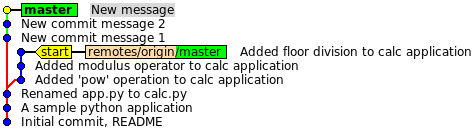
\includegraphics[width=0.75\linewidth]{gitrebase-amend.png}
  \label{fig:gitrebase-amend}
  \caption{Result of amending the last 3 commit messages}
\end{figure*}

\noindent We have covered the general mechanism of git rebase in interactive mode. 
We will now have a small preview of more advances operation which can be done with rebase.
First, let's undo out changes by reset or local master branch to the state of origin/master:

\begin{lstlisting}[style=BashInputStyle]
  git reset --hard origin/master
\end{lstlisting}

\noindent \textbf{Squashing Commits}.
A number of small commits can be combined into one.

This is done using the \textbf{squash} keyword in the git rebase editor.
Let's combine HEAD~1 and HEAD~2:

\begin{lstlisting}[style=BashInputStyle]
  $ git rebase -i HEAD~3
\end{lstlisting}

This time, we modify the rebase editor like the following:
\marginnote{The \textbf{squash} action combines a commit with the previous one, so we need to add squash to the \textbf{lower} element of a pair of commits}
\begin{lstlisting}[style=BashInputStyle]
  pick 21471dd Added 'pow' operation to calc application
  squash 511d31d Added modulus operator to calc application
  pick 87854e9 New message
\end{lstlisting}

When rebasing this, Git first picks 21471dd, then amends it with 511d31d.
An editor opens promoting for the new commit message of the combined commit:
\marginnote{In fact, the squashing in Git is pretty smart: if you squash more than 2 consecutive commits, they will all appear together in this step.}
\begin{lstlisting}[style=BashInputStyle]
# This is a combination of 2 commits.
# The first commit's message is:

Added 'pow' operation to calc application

# This is the 2nd commit message:

Added modulus operator to calc application
\end{lstlisting}

Let's modify it to:

\begin{lstlisting}[style=BashInputStyle]
Added 'pow' and 'modulus' operators
\end{lstlisting}

\begin{lstlisting}[style=BashInputStyle]
  $ git rebase --continue
\end{lstlisting}

The rebase will complete and our new history is shown in Figure \ref{fig:gitrebase-squash}

\begin{figure*}%
  \centering
  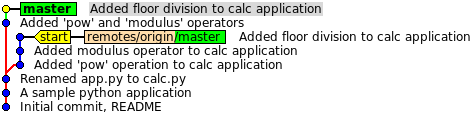
\includegraphics[width=0.75\linewidth]{gitrebase-squash.png}
  \label{fig:gitrebase-squash}
  \caption{Result of a squash in a git rebase}
\end{figure*}

Let's reset our branch again before the next part:

\begin{lstlisting}[style=BashInputStyle]
  git reset --hard origin/master
\end{lstlisting}

\noindent \textbf{Splitting a commit into smaller commits}
Splitting a large commit into smaller ones is also possible, but slightly trickier.
The keyword to use in the interactive rebase editor is \textbf{edit}, just like for editing the commit message.
Suppose we want to split the commit implementing the modulus operation.
We can rebase upto HEAD\textasciitilde2:

\begin{lstlisting}[style=BashInputStyle]
  $ git rebase -i HEAD~2
\end{lstlisting}

In the rebase editor, we \textbf{edit} 511d31d:
\begin{lstlisting}[style=BashInputStyle]
  edit 511d31d Added modulus operator to calc application
  pick 87854e9 New message
\end{lstlisting}

Git will stop after picking 511d31d.
\textbf{The tricky part:} Git has already picked the commit as a whole, the pause is there to add stuff to the staging area and/or edit the commit message.
So how to split it up into smaller ones?
\marginnote{yes, a reset within a rebase operation is allowed}
The user must now \textbf{reset} on HEAD\textasciitilde1, which undoes the last commit, the one Git has just picked, and sets to modified state all the modifications of the commit.

\begin{lstlisting}[style=BashInputStyle]
  $ git reset HEAD~1
\end{lstlisting}

\marginnote{remember how useful git add -p is for staging partial information}
You can now \textbf{git add} the modifications partially, commit, stage more, commit again, etc, until everything has been staged and committed:

\begin{lstlisting}[style=BashInputStyle]
  $ git add -p
  # stage part of the modifications
  $ git commit -m "modulus implementation, phase 1"
  $ git add -p
  # stage part of the modifications
  $ git commit -m "modulus implementation, phase 2"
  $ git rebase --continue
\end{lstlisting}

The local master branch will now contain the split commit:

\begin{figure*}%
  \centering
  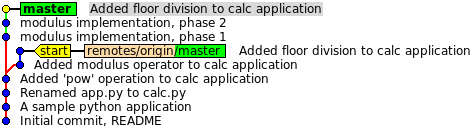
\includegraphics[width=0.75\linewidth]{gitrebase-split.png}
  \label{fig:gitrebase-split}
  \caption{Result of a split in a git rebase}
\end{figure*}

\noindent \textbf{Deleting and Reordering commits}

Finally, it's possible to delete and reorder commits.
To do so, simply delete and reorder lines in the interactive rebase editor.
This is left as exercice.

In the next session, we will dig further into workflows dealing with multiple branches, multiple people, and learn other ways to integrate changes such as \textbf{rebase}.

\bibliography{../common/refs}
\bibliographystyle{plainnat}

\end{document}


% \marginnote{}